\documentclass[11pt]{article}
\usepackage[hmargin=1in,vmargin=1in]{geometry}
\usepackage[document]{ragged2e}
\usepackage{xcolor}
\usepackage{amsmath,amssymb,amsfonts,url,sectsty,framed,tcolorbox,framed}
\usepackage{tikz}
\usepackage{nicematrix}
\newcommand{\pf}{{\bf Proof: }}
\newtheorem{theorem}{Theorem}
\newtheorem{lemma}{Lemma}
\newtheorem{proposition}{Proposition}
\newtheorem{definition}{Definition}
\newtheorem{remark}{Remark}
\newcommand{\qed}{\hfill \rule{2mm}{2mm}}


\begin{document}
%%%%%%%%%%%%%%%%%%%%%%%%%%%%%%%%%%%%%%%%%%%%%%%%%%%%%%%%%%%%%%%%%%%%%
\noindent
\rule{\textwidth}{1pt}
\begin{center}
{\bf [CS304] Introduction to Cryptography and Network Security}
\end{center}
Course Instructor: Dr. Dibyendu Roy \hfill Winter 2022-2023\\
Scribed by: Chitranshi Srivastava (202051055) \hfill Lecture 5 and 6 (Week \#3)
\\
\rule{\textwidth}{1pt}
%%%%%%%%%%%%%%%%%%%%%%%%%%%%%%%%%%%%%%%%%%%%%%%%%%%%%%%%%%%
%write here
In the previous week, we discussed about block ciphers and stream ciphers. We also learnt about One Time Padding(OTP) which we will continue from this session.
\section{One Time Padding (OTP)}
One Time Padding (OTP) provides perfect secrecy under some conditions.\\
\textbf{Encryption: }\\
\vspace{3mm}
$Enc(P, K) = P \oplus K = C$\\
where,\\
 P $\rightarrow$ Plain Text\\
    K $\rightarrow$ Secret Key\\
    $\oplus \rightarrow $ xor operation\\
\vspace{5mm}
\textbf{Decryption: }\\
\vspace{3mm}
    $Dec(C, K) = C \oplus K = P$\\
To ensure that OTP provides perfect secrecy, that is,\\
\begin{center}
    $P(message | Cipher text) = P(message)$
\end{center}
certain conditions have to be fulfilled. These are as follows :
The conditions under which OTP provides perfect secrecy are as follows:
\begin{enumerate}
    \item The secret key K cannot be used to encrypt two messages, that is, the key can not be reused.
    \item The length of key must be greater than or equal to the length of message.\\
    $length(K) \geq length(P)$
    \item Key K is uniformly selected from the key space.
\end{enumerate}
\textbf{Example :}\\
Let us consider OTP on one bit.\\
$message, M\in\{0, 1\} and key, K\in\{0, 1\}$\\
\begin{center}
    $Pr[M = 0] = p$\\
     $Pr[M = 1] = 1-p $
\end{center}
Since we have assumed that key is uniformly selected,
\begin{center}
    Pr[K = 0] = \(\frac{1}{2}\)\\
    \vspace{3mm}
    Pr[K = 1] = \(\frac{1}{2}\)
\end{center}
\vspace{8mm}
\textbf{Encryption :}\\
\begin{center}
    $C = M\oplus K $
\end{center}
Cipher text can be 0 or 1. Let us find the probability.
\begin{center}
    Pr[C = 0] = Pr[M = 0, K = 0] + Pr[M = 1, K = 1]\\
    \vspace{3mm}
    $Pr[C = 0] = Pr[M = 0]\cdot Pr[K = 0] + Pr[M = 1]\cdot Pr[K = 1]$\\
    \vspace{3mm}
    Pr[C = 0] = p$\times$ \(\frac{1}{2}\) + (1-p)$\times$ \(\frac{1}{2}\)\\
    \vspace{3mm}
    \textbf{Pr[C = 0] = \(\frac{1}{2}\)}\\
    \vspace{5mm}
    Pr[C = 1] = 1 - Pr[C = 0]\\
    \vspace{3mm}
    \textbf{Pr[C = 1] = \(\frac{1}{2}\)}\\
\end{center}
Let us prove that OTP with the three conditions stated above provides perfect secrecy.
\begin{center}
    $Pr[M = 0 | C = 0]$ = \(\frac{Pr[M = 0, C = 0]}{Pr[C = 0]}\)\\
    \vspace{5mm}
    $Pr[M = 0 | C = 0]$ = $\frac{Pr[C = 0 | M = 0] \times Pr[M = 0]}{Pr[C = 0]}$\\
\end{center}
    On observing the initial conditions, we see that given that M = 0, it is only possible to get C = 0 iff K = 0. That is, it depends on the probability of K.\\
\begin{center}
    $Pr[M = 0 | C = 0] = \frac{Pr[K = 0] \times Pr[M = 0]}{\frac{1}{2}}$\\
    \vspace{3mm}
    $\textbf{Pr[M = 0 | C = 0] = Pr[M = 0]}$
\end{center}
Since the above condition is proved, we can state that OTP under conditions provides perfect secrecy. This observation can be generalized for any n number of bits.\\
Now let us see how perfect secrecy is not satisfied when the conditions are not fulfilled.
\begin{itemize}
    \item \textbf{When keys for two messages are same :}\\
    \begin{center}
        $M_1 \oplus K = C_1 $\\
        $M_2 \oplus K = C_2 $\\
    \end{center}
    Let us take XOR of both cipher texts
    \begin{center}
        $C_1 \oplus C_2 = (M_1 \oplus K) \oplus (M_2 \oplus K)$\\
        $C_1 \oplus C_2 = M_1 \oplus M_2 $
    \end{center}
    We can see that using the cipher text, we can get information about the difference between the two plain texts. Hence, perfect secrecy is not satisfied.
    \item \textbf{When len(K) $<$ len(P) : }\\
    \vspace{3mm}
    Let us consider len(K) = 16 bits and len(P) = 32 bits
    \begin{center}
        $C = P \oplus K $\\
        \vspace{3mm}
        $C = P \oplus 0000000000000000 k_1...k_{16} $\\
        \vspace{3mm}
        $C = p_1p_2....p_{16}c_{17}...c_{32}$
    \end{center}
    We can see from above that the first 16 bits of plain text will be revealed as zeros will be appended before K to find XOR with P(32 bits) and $A \oplus 0 = A $. Hence, perfect secrecy is not satisfied.\\
    \vspace{5mm}
    If we try to optimize this process by repeating bits of K to avoid taking xor with 0s, even then some information is revealed. Proof is given below. Here, t $<$ n
    \begin{center}
        $P = p_1p_2......p_n$\\
        $K = k_1k_2...k_t$\\
    \end{center}
    Let us repeat bits of k after t length.
    \begin{center}
        $C = (p_1 \oplus k_1)(p_2 \oplus k_2)(p_t \oplus k_t)(p_{t+1} \oplus k_1)...(p_n \oplus k_{n-t})$\\
        Therefore,\\
        $c_1 \oplus c_{t+1} = (p_1 \oplus k_1) \oplus (p_{t+1} \oplus p_1)$\\
        $c_1 \oplus c_{t+1} = p_1 \oplus p_{t+1}$
    \end{center}
    This again reveals information about the plain text. Therefore, perfect secrecy is not satisfied.
\end{itemize}
Hence, we can conclude that the three conditions stated above must be satisfied to attain perfect secrecy in One Time Padding(OTP).
\section{Data Encryption Standard (DES)}
DES is a block cipher designed by IBM. It is based on Feistel Networks. It has the following parameters:
\begin{itemize}
    \item Block Size = 64 bits
    \item Number of Rounds = 16
    \item Secret Key Size = 64 bits (8 parity check bits)
\end{itemize}
\vspace{5mm}
Initially, the design was kept secret and was used for personal communication only. But when the design came into the public domain, the cipher was broken immediately. Several weaknesses revealed the secret key in a short time.\\
\vspace{3mm}
The actual length of secret key is 56 bits. The rest 8 bits are parity bits to ensure the correctness of the main 56 bits.\\
\vspace{3mm}
In sets of 8 bits, the last bit is the parity bit. To find the secret key of DES exhaustively, $2^{56}$ keys will be checked in the worst case.\\
\vspace{5mm}
\textbf{Encryption: }
\begin{center}
    \tikzset{every picture/.style={line width=0.75pt}}  
    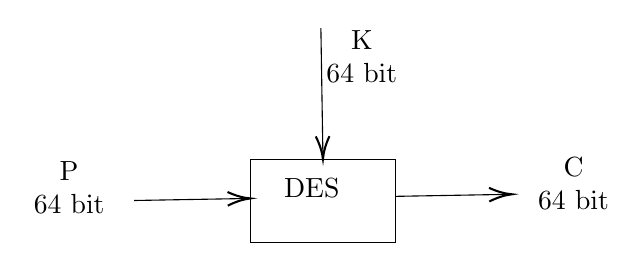
\begin{tikzpicture}[x=0.75pt,y=0.75pt,yscale=-1,xscale=1]
        \draw   (263,99) -- (333,99) -- (333,139) -- (263,139) -- cycle ;
        \draw    (297,35.8) -- (297.97,96.8) ;
        \draw [shift={(298,98.8)}, rotate = 269.09] [color={rgb, 255:red, 0; green, 0; blue, 0 }  ][line width=0.75]    (10.93,-3.29) .. controls (6.95,-1.4) and (3.31,-0.3) .. (0,0) .. controls (3.31,0.3) and (6.95,1.4) .. (10.93,3.29)   ;
        \draw    (207,118.8) -- (261,117.84) ;
        \draw [shift={(263,117.8)}, rotate = 178.98] [color={rgb, 255:red, 0; green, 0; blue, 0 }  ][line width=0.75]    (10.93,-3.29) .. controls (6.95,-1.4) and (3.31,-0.3) .. (0,0) .. controls (3.31,0.3) and (6.95,1.4) .. (10.93,3.29)   ;
        \draw    (333,116.8) -- (387,115.84) ;
        \draw [shift={(389,115.8)}, rotate = 178.98] [color={rgb, 255:red, 0; green, 0; blue, 0 }  ][line width=0.75]    (10.93,-3.29) .. controls (6.95,-1.4) and (3.31,-0.3) .. (0,0) .. controls (3.31,0.3) and (6.95,1.4) .. (10.93,3.29)   ;
        
        \draw (278,107) node [anchor=north west][inner sep=0.75pt]   [align=left] {DES};
        
        \draw (297,35.8) node [anchor=north west][inner sep=0.75pt]   [align=left] {
        \begin{minipage}[lt]{27.68pt}\setlength\topsep{0pt}
            \begin{center}
            K\\64 bit
            \end{center}
        \end{minipage}};
    
        \draw (156,98.8) node [anchor=north west][inner sep=0.75pt]   [align=left] {
        \begin{minipage}[lt]{27.68pt}\setlength\topsep{0pt}
            \begin{center}
            P\\64 bit
            \end{center}
        \end{minipage}};
        
        \draw (399,96.8) node [anchor=north west][inner sep=0.75pt]   [align=left] {
        \begin{minipage}[lt]{27.68pt}\setlength\topsep{0pt}
            \begin{center}
            C\\64 bit
            \end{center}
        \end{minipage}};
    
    \end{tikzpicture}
\end{center}
It takes 64 bit message and a 64 bit key and generates 64 bit cipher text.\\
\vspace{3mm}
\textbf{Decryption:}
\begin{center}
    \tikzset{every picture/.style={line width=0.75pt}}  
    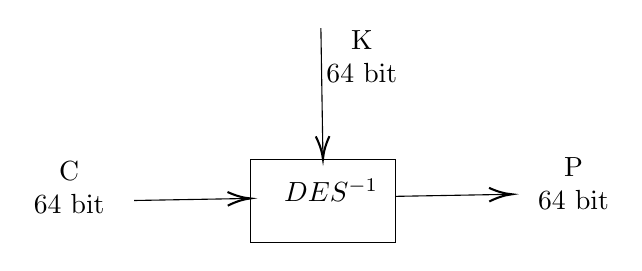
\begin{tikzpicture}[x=0.75pt,y=0.75pt,yscale=-1,xscale=1]
        \draw   (263,99) -- (333,99) -- (333,139) -- (263,139) -- cycle ;
        \draw    (297,35.8) -- (297.97,96.8) ;
        \draw [shift={(298,98.8)}, rotate = 269.09] [color={rgb, 255:red, 0; green, 0; blue, 0 }  ][line width=0.75]    (10.93,-3.29) .. controls (6.95,-1.4) and (3.31,-0.3) .. (0,0) .. controls (3.31,0.3) and (6.95,1.4) .. (10.93,3.29)   ;
        \draw    (207,118.8) -- (261,117.84) ;
        \draw [shift={(263,117.8)}, rotate = 178.98] [color={rgb, 255:red, 0; green, 0; blue, 0 }  ][line width=0.75]    (10.93,-3.29) .. controls (6.95,-1.4) and (3.31,-0.3) .. (0,0) .. controls (3.31,0.3) and (6.95,1.4) .. (10.93,3.29)   ;
        \draw    (333,116.8) -- (387,115.84) ;
        \draw [shift={(389,115.8)}, rotate = 178.98] [color={rgb, 255:red, 0; green, 0; blue, 0 }  ][line width=0.75]    (10.93,-3.29) .. controls (6.95,-1.4) and (3.31,-0.3) .. (0,0) .. controls (3.31,0.3) and (6.95,1.4) .. (10.93,3.29)   ;
        
        \draw (278,107) node [anchor=north west][inner sep=0.75pt]   [align=left] {$DES^{-1}$};
        
        \draw (297,35.8) node [anchor=north west][inner sep=0.75pt]   [align=left] {
        \begin{minipage}[lt]{27.68pt}\setlength\topsep{0pt}
            \begin{center}
            K\\64 bit
            \end{center}
        \end{minipage}};
    
        \draw (156,98.8) node [anchor=north west][inner sep=0.75pt]   [align=left] {
        \begin{minipage}[lt]{27.68pt}\setlength\topsep{0pt}
            \begin{center}
            C\\64 bit
            \end{center}
        \end{minipage}};
        
        \draw (399,96.8) node [anchor=north west][inner sep=0.75pt]   [align=left] {
        \begin{minipage}[lt]{27.68pt}\setlength\topsep{0pt}
            \begin{center}
            P\\64 bit
            \end{center}
        \end{minipage}};
    
    \end{tikzpicture}
\end{center}
The secret key is 64 bits long with every 8th bit (from MSB side) as a parity bit. For Example, 
\begin{center}
    Key: 0110101$\textcolor{red}{0}$ 1101000$\textcolor{red}{1}$ ..... 1101011$\textcolor{red}{1}$
\end{center}
The red coloured bits are parity bits. These are calculated by taking xor of the 7 bits prior to each parity bit. Now, if there is an odd number of bits altered in the 7 bits, it can be identified using the parity bit.\\
\underline{Note}:However, parity bits will not help in identifying an alteration in even number of bits.\\
\vspace{3mm}
The first step of DES is to convert the 65-bit secret key to 56-bit by removing the parity bits. Hence, DES should provide 56-bit security.\\
In DES, there are 16 rounds. DES uses the same round function in every round. For each round, there is a unique round key $K_i$ which is generated by the key scheduling algorithm. The key scheduling algorithm takes secret key as input and generate the round keys $K_1, K_2, ...., K_{16}$, that are of 48 bits.\\
\vspace{3mm}
\textbf{Round Function :}
\begin{center}
    $f: \{0,1\}^{32} \times \{0,1\}^{48} \rightarrow \{0,1\}^{32}$
\end{center}
\textbf{Encryption Algorithm :}\\
\begin{itemize}
    \item We pass the 64-bit input message to the IP which permutes the bits.
    \item The output from IP is then divided into 32-bit left and right halves, $L_0$ and $R_0$
    \item From i = 1 to 16, we execute 16 rounds of fiestal network where,
    \begin{center}
        $L_i = R_{i-1}$
        $R_i = L_{i-1} \oplus f(R_{i-1}, K_i)$
    \end{center}
    where
    \begin{center}
        $f(R_{i-1}, K_i) = P(S(E(R_{i-1} \oplus K_i)))$
    \end{center}
    \item We then exchange $L_{16} $ and $R_{16}$
    \item We then permute the final expression using $IP^{-1}$
\end{itemize}
A flowchart for encrypting a block of message is given below.\\
\begin{center}
    \tikzset{every picture/.style={line width=0.75pt}} 
    
    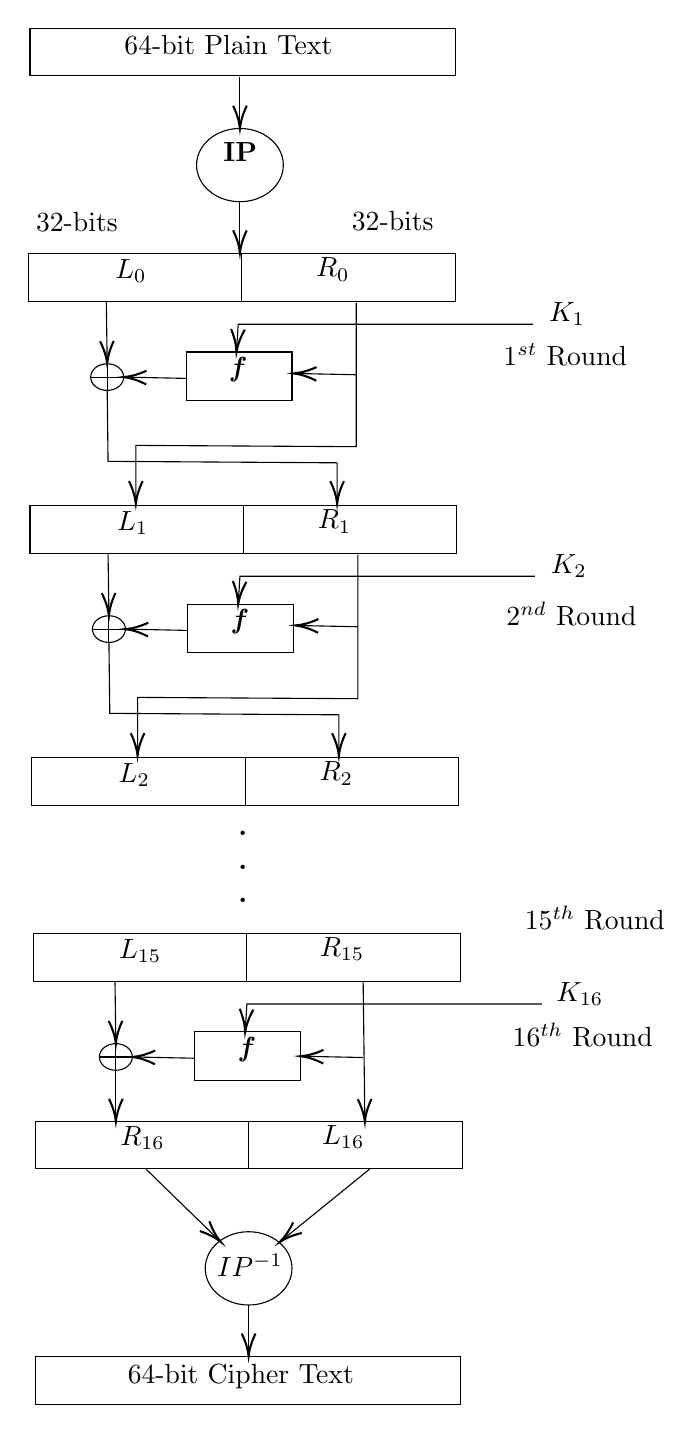
\begin{tikzpicture}[x=0.75pt,y=0.75pt,yscale=-1,xscale=1]
    
    \draw   (192.84,35) -- (397.67,35) -- (397.67,57.87) -- (192.84,57.87) -- cycle ; 
    \draw    (294,58.58) -- (294,81.28) ;
    \draw [shift={(294,83.28)}, rotate = 270] [color={rgb, 255:red, 0; green, 0; blue, 0 }  ][line width=0.75]    (10.93,-3.29) .. controls (6.95,-1.4) and (3.31,-0.3) .. (0,0) .. controls (3.31,0.3) and (6.95,1.4) .. (10.93,3.29)   ; 
    \draw   (273.1,100.93) .. controls (273.1,91.19) and (282.46,83.28) .. (294,83.28) .. controls (305.54,83.28) and (314.9,91.19) .. (314.9,100.93) .. controls (314.9,110.68) and (305.54,118.58) .. (294,118.58) .. controls (282.46,118.58) and (273.1,110.68) .. (273.1,100.93) -- cycle ;
    \draw   (192,143.71) -- (294.84,143.71) -- (294.84,166.58) -- (192,166.58) -- cycle ;
    \draw    (294,118.58) -- (294,141.29) ;
    \draw [shift={(294,143.29)}, rotate = 270] [color={rgb, 255:red, 0; green, 0; blue, 0 }  ][line width=0.75]    (10.93,-3.29) .. controls (6.95,-1.4) and (3.31,-0.3) .. (0,0) .. controls (3.31,0.3) and (6.95,1.4) .. (10.93,3.29)   ;
    \draw   (294.84,143.71) -- (397.67,143.71) -- (397.67,166.58) -- (294.84,166.58) -- cycle ;
    \draw   (268.08,191.01) -- (319.08,191.01) -- (319.08,214.44) -- (268.08,214.44) -- cycle ; 
    \draw   (222.1,203.08) .. controls (222.1,199.53) and (225.65,196.66) .. (230.04,196.66) .. controls (234.43,196.66) and (237.98,199.53) .. (237.98,203.08) .. controls (237.98,206.63) and (234.43,209.5) .. (230.04,209.5) .. controls (225.65,209.5) and (222.1,206.63) .. (222.1,203.08) -- cycle ; \draw   (222.1,203.08) -- (237.98,203.08) ; \draw   (230.04,196.66) -- (230.04,209.5) ;
    \draw    (350.02,167.29) -- (350.02,236.61) -- (253.87,236.04) -- (243.84,235.98) -- (243.84,262.14) ;
    \draw [shift={(243.84,264.14)}, rotate = 270] [color={rgb, 255:red, 0; green, 0; blue, 0 }  ][line width=0.75]    (10.93,-3.29) .. controls (6.95,-1.4) and (3.31,-0.3) .. (0,0) .. controls (3.31,0.3) and (6.95,1.4) .. (10.93,3.29)   ;
    \draw   (192.84,265.13) -- (295.67,265.13) -- (295.67,288) -- (192.84,288) -- cycle ;
    \draw   (295.67,265.13) -- (398.51,265.13) -- (398.51,288) -- (295.67,288) -- cycle ;
    \draw    (350.02,201.95) -- (321.92,201.36) ;
    \draw [shift={(319.92,201.31)}, rotate = 1.21] [color={rgb, 255:red, 0; green, 0; blue, 0 }  ][line width=0.75]    (10.93,-3.29) .. controls (6.95,-1.4) and (3.31,-0.3) .. (0,0) .. controls (3.31,0.3) and (6.95,1.4) .. (10.93,3.29)   ;
    \draw    (268.08,203.71) -- (239.98,203.12) ;
    \draw [shift={(237.98,203.08)}, rotate = 1.21] [color={rgb, 255:red, 0; green, 0; blue, 0 }  ][line width=0.75]    (10.93,-3.29) .. controls (6.95,-1.4) and (3.31,-0.3) .. (0,0) .. controls (3.31,0.3) and (6.95,1.4) .. (10.93,3.29)   ;
    \draw    (229.62,166.58) -- (230.01,194.66) ;
    \draw [shift={(230.04,196.66)}, rotate = 269.2] [color={rgb, 255:red, 0; green, 0; blue, 0 }  ][line width=0.75]    (10.93,-3.29) .. controls (6.95,-1.4) and (3.31,-0.3) .. (0,0) .. controls (3.31,0.3) and (6.95,1.4) .. (10.93,3.29)   ; 
    \draw    (230.04,209.5) -- (230.46,243.67) -- (340.82,244.38) -- (340.82,262.14) ;
    \draw [shift={(340.82,264.14)}, rotate = 270] [color={rgb, 255:red, 0; green, 0; blue, 0 }  ][line width=0.75]    (10.93,-3.29) .. controls (6.95,-1.4) and (3.31,-0.3) .. (0,0) .. controls (3.31,0.3) and (6.95,1.4) .. (10.93,3.29)   ;
    \draw    (435.3,177.6) -- (293.16,177.6) -- (292.45,189.01) ;
    \draw [shift={(292.33,191.01)}, rotate = 273.57] [color={rgb, 255:red, 0; green, 0; blue, 0 }  ][line width=0.75]    (10.93,-3.29) .. controls (6.95,-1.4) and (3.31,-0.3) .. (0,0) .. controls (3.31,0.3) and (6.95,1.4) .. (10.93,3.29)   ;
    \draw   (268.92,312.43) -- (319.92,312.43) -- (319.92,335.86) -- (268.92,335.86) -- cycle ; 
    \draw   (222.93,324.5) .. controls (222.93,320.95) and (226.49,318.07) .. (230.88,318.07) .. controls (235.26,318.07) and (238.82,320.95) .. (238.82,324.5) .. controls (238.82,328.05) and (235.26,330.92) .. (230.88,330.92) .. controls (226.49,330.92) and (222.93,328.05) .. (222.93,324.5) -- cycle ; \draw   (222.93,324.5) -- (238.82,324.5) ; \draw   (230.88,318.07) -- (230.88,330.92) ;
    \draw    (350.85,288.71) -- (350.85,358.03) -- (254.71,357.46) -- (244.67,357.4) -- (244.67,383.56) ;
    \draw [shift={(244.67,385.56)}, rotate = 270] [color={rgb, 255:red, 0; green, 0; blue, 0 }  ][line width=0.75]    (10.93,-3.29) .. controls (6.95,-1.4) and (3.31,-0.3) .. (0,0) .. controls (3.31,0.3) and (6.95,1.4) .. (10.93,3.29)   ; 
    \draw   (193.67,386.55) -- (296.51,386.55) -- (296.51,409.42) -- (193.67,409.42) -- cycle ;
    \draw   (296.51,386.55) -- (399.35,386.55) -- (399.35,409.42) -- (296.51,409.42) -- cycle ;
    \draw    (350.85,323.37) -- (322.75,322.78) ;
    \draw [shift={(320.76,322.73)}, rotate = 1.21] [color={rgb, 255:red, 0; green, 0; blue, 0 }  ][line width=0.75]    (10.93,-3.29) .. controls (6.95,-1.4) and (3.31,-0.3) .. (0,0) .. controls (3.31,0.3) and (6.95,1.4) .. (10.93,3.29)   ; 
    \draw    (268.92,325.13) -- (240.82,324.54) ;
    \draw [shift={(238.82,324.5)}, rotate = 1.21] [color={rgb, 255:red, 0; green, 0; blue, 0 }  ][line width=0.75]    (10.93,-3.29) .. controls (6.95,-1.4) and (3.31,-0.3) .. (0,0) .. controls (3.31,0.3) and (6.95,1.4) .. (10.93,3.29)   ;
    \draw    (230.46,288) -- (230.85,316.07) ;
    \draw [shift={(230.88,318.07)}, rotate = 269.2] [color={rgb, 255:red, 0; green, 0; blue, 0 }  ][line width=0.75]    (10.93,-3.29) .. controls (6.95,-1.4) and (3.31,-0.3) .. (0,0) .. controls (3.31,0.3) and (6.95,1.4) .. (10.93,3.29)   ;
    \draw    (230.88,330.92) -- (231.3,365.09) -- (341.66,365.79) -- (341.66,383.56) ;
    \draw [shift={(341.66,385.56)}, rotate = 270] [color={rgb, 255:red, 0; green, 0; blue, 0 }  ][line width=0.75]    (10.93,-3.29) .. controls (6.95,-1.4) and (3.31,-0.3) .. (0,0) .. controls (3.31,0.3) and (6.95,1.4) .. (10.93,3.29)   ;
    \draw    (436.13,299.01) -- (294,299.01) -- (293.29,310.43) ;
    \draw [shift={(293.16,312.43)}, rotate = 273.57] [color={rgb, 255:red, 0; green, 0; blue, 0 }  ][line width=0.75]    (10.93,-3.29) .. controls (6.95,-1.4) and (3.31,-0.3) .. (0,0) .. controls (3.31,0.3) and (6.95,1.4) .. (10.93,3.29)   ;
    \draw   (194.51,471.26) -- (297.35,471.26) -- (297.35,494.13) -- (194.51,494.13) -- cycle ; 
    \draw   (297.35,471.26) -- (400.18,471.26) -- (400.18,494.13) -- (297.35,494.13) -- cycle ;
    \draw   (272.26,518.56) -- (323.26,518.56) -- (323.26,541.99) -- (272.26,541.99) -- cycle ;
    \draw   (226.28,530.63) .. controls (226.28,527.08) and (229.84,524.2) .. (234.22,524.2) .. controls (238.61,524.2) and (242.16,527.08) .. (242.16,530.63) .. controls (242.16,534.17) and (238.61,537.05) .. (234.22,537.05) .. controls (229.84,537.05) and (226.28,534.17) .. (226.28,530.63) -- cycle ; \draw   (226.28,530.63) -- (242.16,530.63) ; \draw   (234.22,524.2) -- (234.22,537.05) ;
    \draw    (233.8,494.13) -- (234.19,522.2) ;
    \draw [shift={(234.22,524.2)}, rotate = 269.2] [color={rgb, 255:red, 0; green, 0; blue, 0 }  ][line width=0.75]    (10.93,-3.29) .. controls (6.95,-1.4) and (3.31,-0.3) .. (0,0) .. controls (3.31,0.3) and (6.95,1.4) .. (10.93,3.29)   ;
    \draw    (439.48,505.14) -- (297.35,505.14) -- (296.63,516.56) ;
    \draw [shift={(296.51,518.56)}, rotate = 273.57] [color={rgb, 255:red, 0; green, 0; blue, 0 }  ][line width=0.75]    (10.93,-3.29) .. controls (6.95,-1.4) and (3.31,-0.3) .. (0,0) .. controls (3.31,0.3) and (6.95,1.4) .. (10.93,3.29)   ;
    \draw   (195.34,561.62) -- (298.18,561.62) -- (298.18,584.49) -- (195.34,584.49) -- cycle ;
    \draw   (298.18,561.62) -- (401.02,561.62) -- (401.02,584.49) -- (298.18,584.49) -- cycle ;
    \draw    (353.36,530.91) -- (325.26,530.32) ;
    \draw [shift={(323.26,530.27)}, rotate = 1.21] [color={rgb, 255:red, 0; green, 0; blue, 0 }  ][line width=0.75]    (10.93,-3.29) .. controls (6.95,-1.4) and (3.31,-0.3) .. (0,0) .. controls (3.31,0.3) and (6.95,1.4) .. (10.93,3.29)   ;
    \draw    (353.36,494.13) -- (354.17,559.9) ;
    \draw [shift={(354.2,561.9)}, rotate = 269.29] [color={rgb, 255:red, 0; green, 0; blue, 0 }  ][line width=0.75]    (10.93,-3.29) .. controls (6.95,-1.4) and (3.31,-0.3) .. (0,0) .. controls (3.31,0.3) and (6.95,1.4) .. (10.93,3.29)   ;
    \draw    (234.22,537.05) -- (234.22,559.76) ;
    \draw [shift={(234.22,561.76)}, rotate = 270] [color={rgb, 255:red, 0; green, 0; blue, 0 }  ][line width=0.75]    (10.93,-3.29) .. controls (6.95,-1.4) and (3.31,-0.3) .. (0,0) .. controls (3.31,0.3) and (6.95,1.4) .. (10.93,3.29)   ;
    \draw   (277.28,632.49) .. controls (277.28,622.74) and (286.64,614.84) .. (298.18,614.84) .. controls (309.73,614.84) and (319.08,622.74) .. (319.08,632.49) .. controls (319.08,642.24) and (309.73,650.14) .. (298.18,650.14) .. controls (286.64,650.14) and (277.28,642.24) .. (277.28,632.49) -- cycle ; 
    \draw    (248.85,584.77) -- (283.37,618.39) ;
    \draw [shift={(284.8,619.78)}, rotate = 224.24] [color={rgb, 255:red, 0; green, 0; blue, 0 }  ][line width=0.75]    (10.93,-3.29) .. controls (6.95,-1.4) and (3.31,-0.3) .. (0,0) .. controls (3.31,0.3) and (6.95,1.4) .. (10.93,3.29)   ;
    \draw    (356.71,584.49) -- (314.78,618.52) ;
    \draw [shift={(313.23,619.78)}, rotate = 320.93] [color={rgb, 255:red, 0; green, 0; blue, 0 }  ][line width=0.75]    (10.93,-3.29) .. controls (6.95,-1.4) and (3.31,-0.3) .. (0,0) .. controls (3.31,0.3) and (6.95,1.4) .. (10.93,3.29)   ; 
    \draw    (298.18,650.14) -- (298.18,672.85) ;
    \draw [shift={(298.18,674.85)}, rotate = 270] [color={rgb, 255:red, 0; green, 0; blue, 0 }  ][line width=0.75]    (10.93,-3.29) .. controls (6.95,-1.4) and (3.31,-0.3) .. (0,0) .. controls (3.31,0.3) and (6.95,1.4) .. (10.93,3.29)   ;
    \draw   (195.34,675.13) -- (400.18,675.13) -- (400.18,698) -- (195.34,698) -- cycle ;
    \draw    (272.26,531.26) -- (244.16,530.67) ;
    \draw [shift={(242.16,530.63)}, rotate = 1.21] [color={rgb, 255:red, 0; green, 0; blue, 0 }  ][line width=0.75]    (10.93,-3.29) .. controls (6.95,-1.4) and (3.31,-0.3) .. (0,0) .. controls (3.31,0.3) and (6.95,1.4) .. (10.93,3.29)   ;
    
    \draw (237.08,37.29) node [anchor=north west][inner sep=0.75pt]   [align=left] {64-bit Plain Text};
    \draw (284.76,88.65) node [anchor=north west][inner sep=0.75pt]   [align=left] {\textbf{IP}};
    \draw (232.67,145.12) node [anchor=north west][inner sep=0.75pt]   [align=left] {$L_0$};
    \draw (329.49,144.42) node [anchor=north west][inner sep=0.75pt]   [align=left] {$R_0$};
    \draw (194.51,122.53) node [anchor=north west][inner sep=0.75pt]   [align=left] {32-bits};
    \draw (346.67,121.83) node [anchor=north west][inner sep=0.75pt]   [align=left] {32-bits};
    \draw (288.51,192.42) node [anchor=north west][inner sep=0.75pt]   [align=left] {\textbf{\textit{f}}};
    \draw (233.51,266.54) node [anchor=north west][inner sep=0.75pt]   [align=left] {$L_1$};
    \draw (330.33,265.84) node [anchor=north west][inner sep=0.75pt]   [align=left] {$R_1$};
    \draw (441.71,165.88) node [anchor=north west][inner sep=0.75pt]   [align=left] {$K_1$};
    \draw (419.71,185.7) node [anchor=north west][inner sep=0.75pt]   [align=left] {$1^{st}$ Round};
    \draw (289.35,313.84) node [anchor=north west][inner sep=0.75pt]   [align=left] {\textbf{\textit{f}}};
    \draw (234.34,387.96) node [anchor=north west][inner sep=0.75pt]   [align=left] {$L_2$};
    \draw (331.17,387.25) node [anchor=north west][inner sep=0.75pt]   [align=left] {$R_2$};
    \draw (442.54,287.3) node [anchor=north west][inner sep=0.75pt]   [align=left] {$K_2$};
    \draw (421.13,310.12) node [anchor=north west][inner sep=0.75pt]   [align=left] {$2^{nd}$ Round};
    \draw (234.53,472.67) node [anchor=north west][inner sep=0.75pt]   [align=left] {$L_{15}$};
    \draw (331.26,471.97) node [anchor=north west][inner sep=0.75pt]   [align=left] {$R_{15}$};
    \draw (430,456.72) node [anchor=north west][inner sep=0.75pt]   [align=left] {$15^{th}$ Round};
    \draw (292.69,519.97) node [anchor=north west][inner sep=0.75pt]   [align=left] {\textbf{\textit{f}}};
    \draw (445.23,493.43) node [anchor=north west][inner sep=0.75pt]   [align=left] {$K_{16}$};
    \draw (424.15,513.25) node [anchor=north west][inner sep=0.75pt]   [align=left] {$16^{th}$ Round};
    \draw (235.12,563.03) node [anchor=north west][inner sep=0.75pt]   [align=left] {$R_{16}$};
    \draw (332.35,562.32) node [anchor=north west][inner sep=0.75pt]   [align=left] {$L_{16}$};
    \draw (281.79,624.21) node [anchor=north west][inner sep=0.75pt]   [align=left] {\textbf{$IP^{-1}$}};
    \draw (238.69,677.42) node [anchor=north west][inner sep=0.75pt]   [align=left] {64-bit Cipher Text};
    \draw (292,420.8) node [anchor=north west][inner sep=0.75pt]   [align=left] {\textbf{.}\\\textbf{.}\\\textbf{.}\\};
\end{tikzpicture}
\end{center}
Here, IP is the Initial Permutation.\\
\vspace{3mm}
Similar to Feistel Network, for each round $L_{i+1}$ and $R_{i+1}$ will be:
\begin{center}
    $L_{i+1} = R_i$\\
    $R_{i+1} = L_i \oplus f(R_i, K_{i+1})$
\end{center}
where $i \in \{0, 1,..., 15\}$. In the last round, i.e. $16^{th}$ round, the position of $L_{16}$ and $R_{16}$ are swapped. After this round, the inverse of Initial Permutation ($IP^{-1}$) is applied to the 64-bits and we get the cipher text.\\
\newline
We need to address the following now:
\begin{itemize}
    \item Initial Permutation and its inverse
    \item The round function $f$
    \item How are the round keys $K_1, K_2, ...., K_{16}$ generated.
\end{itemize}
\subsection{Initial Permutation}
It is a bijection from 64-bit to 64-bit. The 64-bit message is permuted using the IP and then further encryption is done. Initial Permutation is defined as:
\begin{center}
IP =  
    $\begin{bmatrix}
    58 & 50 & 42 & 34 & 26 & 18 & 10 & 2\\
    60 & 52 & 44 & 36 & 28 & 20 & 12 & 4\\
    62 & 54 & 46 & 38 & 30 & 22 & 14 & 6\\
    64 & 56 & 48 & 40 & 32 & 24 & 16 & 8\\
    57 & 49 & 41 & 33 & 25 & 17 & 9 & 1\\
    59 & 51 & 43 & 35 & 27 & 19 & 11 & 3\\
    61 & 53 & 45 & 37 & 29 & 21 & 13 & 5\\
    63 & 55 & 47 & 39 & 31 & 23 & 25 & 7\\
    \end{bmatrix}$
\end{center}
The permutation can be simply visualised as:
\begin{center}
    $IP(m_1m_2...m_7m_8m_9....m_{64}) = m_{58}m_{50}...m_{10}m_2m_{60}....m_7 $
\end{center}
We can easily compute its inverse and it will be equal to:
\begin{center}
    $IP^{-1} = 
    \begin{bmatrix}
        40 & 8 & 48 & 16 & 56 & 24 & 64 & 32\\
        39 & 7 & 47 & 15 & 55 & 23 & 63 & 31\\
        38 & 6 & 46 & 14 & 54 & 22 & 62 & 30\\
        37 & 5 & 45 & 13 & 53 & 21 & 61 & 29\\
        36 & 4 & 44 & 12 & 52 & 20 & 60 & 28\\
        35 & 3 & 43 & 11 & 51 & 19 & 59 & 27\\
        34 & 2 & 42 & 10 & 50 & 18 & 58 & 26\\
        33 & 1 & 41 & 9 & 49 & 17 & 57 & 25\\
    \end{bmatrix}$
\end{center}
\subsection{Round Function of DES}
\begin{center}
    $f: \{0,1\}^{32} \times \{0,1\}^{48} \rightarrow \{0,1\}^{32}$\\
    $f(R_i, K_i) = X_i$\\
    where,\\
    $R_i$ is 32-bit\\
    $K_i$ is 48-bit\\
    $X_i$ is 32-bit.
\end{center}
The round function for DES is defined as:
\begin{center}
    $f(R_i, K_i) = P(S(E(R_i) \oplus K_i))$\\
\end{center}
where,\\
    Expansion Function E : $\{0, 1\}^{32} \rightarrow \{0, 1\}^{48}$\\
    Substitution Box S: $\{0, 1\}^{48} \rightarrow \{0, 1\}^{32}$\\
    Permutation Box P: $\{0, 1\}^{32} \rightarrow \{0, 1\}^{32}$\\
Hence,
\begin{center}
    length of $R_i$ = 32-bits\\
    length of $E(R_i)$ = 48-bits = length of $K_i$\\
    length of $E(R_i) \oplus K_i$ = 48-bits\\
    length of $S(E(R_i) \oplus K_i)$ = 32-bits\\
    length of $P(S(E(R_i) \oplus K_i))$ = 32-bits
\end{center}
\subsubsection{Expansion Function}
\begin{center}
    $E: \{0, 1\}^{32} \rightarrow \{0, 1\}^{48}$\\    
\end{center}

The expansion function for DES is given below:
\begin{center}
    $ E = 
    \begin{bmatrix}
        32 & 1 & 2 & 3 & 4 & 5\\
        4 & 5 & 6 & 7 & 8 & 9\\
        8 & 9 & 10 & 11 & 12 & 13\\
        12 & 13 & 14 & 15 & 16 & 17\\
        16 & 17 & 18 & 19 & 20 & 21\\
        20 & 21 & 22 & 23 & 24 & 25\\
        24 & 25 & 26 & 27 & 28 & 29\\
        28 & 29 & 30 & 31 & 32 & 1\\
    \end{bmatrix}$
\end{center}
The bits are repeated for expanding 32-bits to 48-bits.
In simple words, for each set of 4 bits, we add the LSB of prev set in the beginning of current set and the MSB of next set at the end of current set. We do in a circular manner for the first and last set.
\begin{center}
    $E(x_1x_2....x_{32}) = (x_{32}x_1x_2x_3x_4x_5x_4x_5....x_{32}x_1)$
\end{center}
\subsubsection{Substitution Box}
\begin{center}
    $S: \{0, 1\}^{48} \rightarrow \{0, 1\}^{32}$\\
    $S(X) = Y$,  where X is 48 and Y is 32 bit long
\end{center}
Dividing X into 8 parts each of length 6-bits.
\begin{center}
    $X = B_1B_2B_3B_4B_5B_6B_7B_8$\\
\end{center}
Corresponding to each $B_i$ there is a substitution box $S_i$ where $i \in \{1,2,..,8\}$.
\begin{center}
    $S_i: \{0, 1\}^6 \rightarrow \{0, 1\}^4  \forall i \in \{1,2,..,8\}$\\
    $S_i(B_i) = C_i$\\
    $\therefore S(X) = (S_1(B_1), S_2(B_2), S_3(B_3), S_4(B_4), S_5(B_5), S_6(B_6), S_7(B_7), S_8(B_8))$ 
\end{center}
Therefore, length of S(X) is 32 bits.
\vspace{3mm}
The substitution boxes are given on page 260 of the book \'Handbook of Applied Cryptography\'. Now let us see how to perform the conversion using Substitution box.\\
\begin{center}
    $B_i = b_1b_2b_3b_4b_5b_6$ , where $b_i \in \{0,1\} $
\end{center}
We can find the row and column of the substitution box using these bits.\\
\begin{center}
    r(row) = $2*b_1 + b_6$, \\
    where r is integer representation of $b_1b_6$  and $0 \leq r \leq 3 $\\
\end{center}
\begin{center}
    c(column) = integer representation of $b_2b_3b_4b_5$\\
    where $0 \leq c \leq  15 $
\end{center}
\begin{center}
    $ S_i = 
    \begin{bmatrix}
        a_{0,0} & \dots & a_{0,15}\\
        \vdots & \ddots & \vdots\\
        a_{3,0} & \dots & a_{3,15}\\
    \end{bmatrix}$ 
    where $a_{i,j} \in \{0, 1,...15\}$
\end{center}
now using this $S_i$ :
\begin{center}
    $S_i(B_i) = a_{r,c}$
\end{center}
\subsubsection{Permutation Box}
\begin{center}
    $P: \{0, 1\}^{32} \rightarrow \{0, 1\}^{32}$\\
\end{center}
It is also defined by a table. The table is given below:
\begin{center}
    $ P = 
    \begin{bmatrix}
        16 && 7 && 20 && 21\\
        29 && 12 && 28 && 17\\
        1 && 15 && 23 && 26\\
        5 && 18 && 31 && 10\\
        2 && 8 && 24 && 14\\
        32 && 27 && 3 && 9\\
        19 && 13 && 30 && 6\\
        22 && 11 && 4 && 25\\
    \end{bmatrix}$
\end{center}
Using this, we can see the permutation as:
\begin{center}
    $P(x_1x_2x_3x_4x_5...x_{32}) = x_{16}x_7x_{20}x_{21}x_{29}...x_{25}$
\end{center}
\subsection{Key Scheduling Algorithm}
\textbf{Input : } 64-bit secret key\\
\textbf{Output : } 16 round keys where len($k_i) = 48 $ bits\\
\vspace{3mm}
\textbf{Algorithm :}
\begin{itemize}
    \item Define $v_i, 1 \leq i \leq 16$, where $v_i = 1$ if $i \in \{1, 2, 9, 16\}$, else $v_i = 2$. 
    \item Discard 8 parity check bits from K. The 56 bit key is \~{K}.
    \item T = PC1(\~{K}), where PC1 is a permuation defined as:
    \begin{center}
        $PC1: \{0, 1\}^{56} \rightarrow \{0, 1\}^{56}$\\
    \end{center}

    \item $(C_0, D_0) = T$, where $C_0$ is most significant 28 bits of T and $D_0$ is least significant 28 bits of T.

    \item for $i = 1$ to 16:
    \begin{center}
        $C_i = (C_{i-1} \hookleftarrow v_i)$\\
        $D_i = (D_{i-1} \hookleftarrow v_i)$\\
        where $\hookleftarrow$ is left circular shift\\
        For example: $x_1x_2x_3....x_28 \hookleftarrow 2 = x_3x_4x_5....x_1x_2 $
        $K_i = PC2(C_i, D_i)$\\
    \end{center}
    where, PC2 is a substitution defined as:
    \begin{center}
        $PC2: \{0, 1\}^{56} \rightarrow \{0, 1\}^{48}$\\
    \end{center}
\end{itemize}
\subsubsection{PC1(Permuted Choice 1)}
It permutes the 56 bits of secret key before generating round keys.
\begin{center}
        $PC1: \{0, 1\}^{56} \rightarrow \{0, 1\}^{56}$\\
\end{center}
\textbf{For $C_i$:}\\
\begin{center}
PC1 = 
$\begin{bmatrix}
    57 & 49 & 41 & 33 & 25 & 17 & 9\\
    1 & 58 & 50 & 42 & 34 & 26 & 18\\
    10 & 2 & 59 & 51 & 43 & 35 & 27\\
    19 & 11 & 3 & 60 & 52 & 44 & 36\\
\end{bmatrix}$
\end{center}
\textbf{For $D_i$:}\\
\begin{center}
PC1 = 
$\begin{bmatrix}
    63 & 55 & 47 & 39 & 31 & 23 & 15\\
    7 & 62 & 54 & 46 & 38 & 30 & 22\\
    14 & 6 & 61 & 53 & 45 & 37 & 29\\
    21 & 13 & 5 & 28 & 20 & 12 & 4\\
\end{bmatrix}$
\end{center}
\begin{center}
    $PC1(k_1k_2\dots k_7k_9\dots k_{63}) = (k_{57}k_{49}k_{41}k_{33}\dots k_9k_1k_{58}\dots k_{63}k_{55}\dots k_4)$
\end{center}
\subsubsection{PC2(Permuted Choice 2)}
It is used to select 48 bits from the concatenation $ b_1b_2 \dots b_{56}$ of $C_i$ and $D_i$\\
\begin{center}
    PC2 = 
    \begin{bmatrix}
        14 & 17 & 11 & 24 & 1 & 5\\
        3 & 28 & 15 & 6 & 21 & 10\\
        23 & 19 & 12 & 4 & 26 & 8\\
        16 & 7 & 27 & 20 & 13 & 2\\
        41 & 52 & 31 & 37 & 47 & 55\\
        30 & 40 & 51 & 45 & 33 & 48\\
        44 & 49 & 39 & 56 & 34 & 53\\
        46 & 42 & 50 & 36 & 29 & 32\\
    \end{bmatrix}
\end{center}
\begin{center}
    $K_i = b_{14}b_{17}b_{11}\dots b_32 $
\end{center}
\subsection{Complementarity Property of DES}
We know that in expansion function, we simply use the bits and map them using the expansion table. Hence, taking complement after mapping is same as mapping the complemented bits. Therefore, 
\begin{center}
    $E(\overline{R_0}) \oplus \overline{K} = \overline{E(R_0)} \oplus \overline{K}$\\
\end{center}
Therefore,
\begin{center}
    $P(S(E(\overline{R_0}) \oplus \overline{K})) = P(S(\overline{E(R_0)} \oplus \overline{K}))$\\
    \vspace{5mm}
    \textbf{$\Rightarrow f(R_0, K) = f(\overline{R_0}, \overline{K})$}
\end{center}
Now let us see for message M, key K :
\begin{center}
    $M = L_0 \parallel R_0$\\
    $L_1 = R_0$\\
    $R_1 = L_0 \oplus f(R_0, K)$\\
    $C = L1 \parallel R_1$\\
\end{center}
For message $\overline{M}, key \overline{K}$, where  $\overline{M}$ and $\overline{K}$ are complements of M and K respectively:
\begin{center}
    $\overline{M} = \overline{L_0} \parallel \overline{R_0}$\\
    $ \tilde{L_1} = \overline{R_0}$\\
    $ \tilde{R_1} = \overline{L_0} \oplus f(\overline{R_0}, \overline{K})$\\
\end{center}
But we proved above that: $f(R_0, K) = f(\overline{R_0}, \overline{K})$.\\ Hence,
\begin{center}
    $\tilde{R_1} = \overline{L_0} \oplus f(R_0, K)$\\
    We also know that $\overline{A} \oplus B = \overline{A \oplus B}$. So, \\
    $\tilde{R_1} = \overline{L_0 \oplus f(R_0, K)}$\\
    $\tilde{R_1} = \overline{R1}$
\end{center}
We can conclude :
\begin{center}
    $\tilde{L_1} \parallel \tilde{R_1} = \overline{L_1} \parallel \overline{R_1}$\\
    \vspace{5mm}
    $\Rightarrow \tilde{C} = \overline{C}$
\end{center}
The proof that we have seen above is for round. But if we consider the whole process of DES, if the secret key K is complemented, the round keys $K_i$ will also be complemented because they are the permutations of secret key K. For the next round, the input will be $\overline{C_1}$ and $\overline{K_2}$. So it will generate output as $\overline{C_2}$. Similarly, after all 16 rounds also, this complementarity property will hold. And in the final step, $IP^{-1}$ also performs permutation, which again maintains complementarity.
\end{document}